\documentclass[11pt]{beamer}
\usetheme{Warsaw}
\usepackage[utf8]{inputenc}
\usepackage[T1]{fontenc}
\usepackage[english]{babel}
\usepackage{amsmath}
\usepackage{amsfonts}
\usepackage{amssymb}
\usepackage{graphicx}
\author{
	Author:Paweł Otrębski \and \\
	 Supervisor: Dr Wojciech Macyna
}
\title{Web based Estate Agent}

%\setbeamercovered{transparent} 
%\setbeamertemplate{navigation symbols}{} 
%\logo{} 
\institute{Wroclaw University of Technology} 
\date{} 
\subject{Undergraduate Project} 
\begin{document}

\begin{frame}{}
\titlepage
\end{frame}

\begin{frame}
\tableofcontents
\end{frame}

\begin{frame}{Introduction}
% This is the introductory frame, that explains the aim
% of the project, what it is that we are trying to achieve 
% note speak of the need to verify 
\begin{flushleft}
\textbf{Aim}\\
\pause
\begin{itemize}
	\item Advertise sundry living space
	\pause
	\item Expose offers to users
	\pause
	\item Rudimentary management for clients and admins 
	\pause
	\begin{itemize}
		\item bookings 
		\item confirmations
		\item cancellations
	\end{itemize}
	\pause
	\item Rate experience minimize/mitigate spamming
	\pause
	\item API that is front end agnostic
\end{itemize}
\end{flushleft}
\end{frame}

\begin{frame}{Motivation}
	\begin{flushleft}
	\textbf{Key motivations}
	\begin{itemize}
		\item sorting by price %watch out for 'sorting' questions
		\item avoid formal accommodation services
		\item build a personal relationship
		\item client feedback
		\item rate a client
	\end{itemize}
	\end{flushleft}
\end{frame}

\begin{frame}{Users and Use cases}
	\begin{figure}
		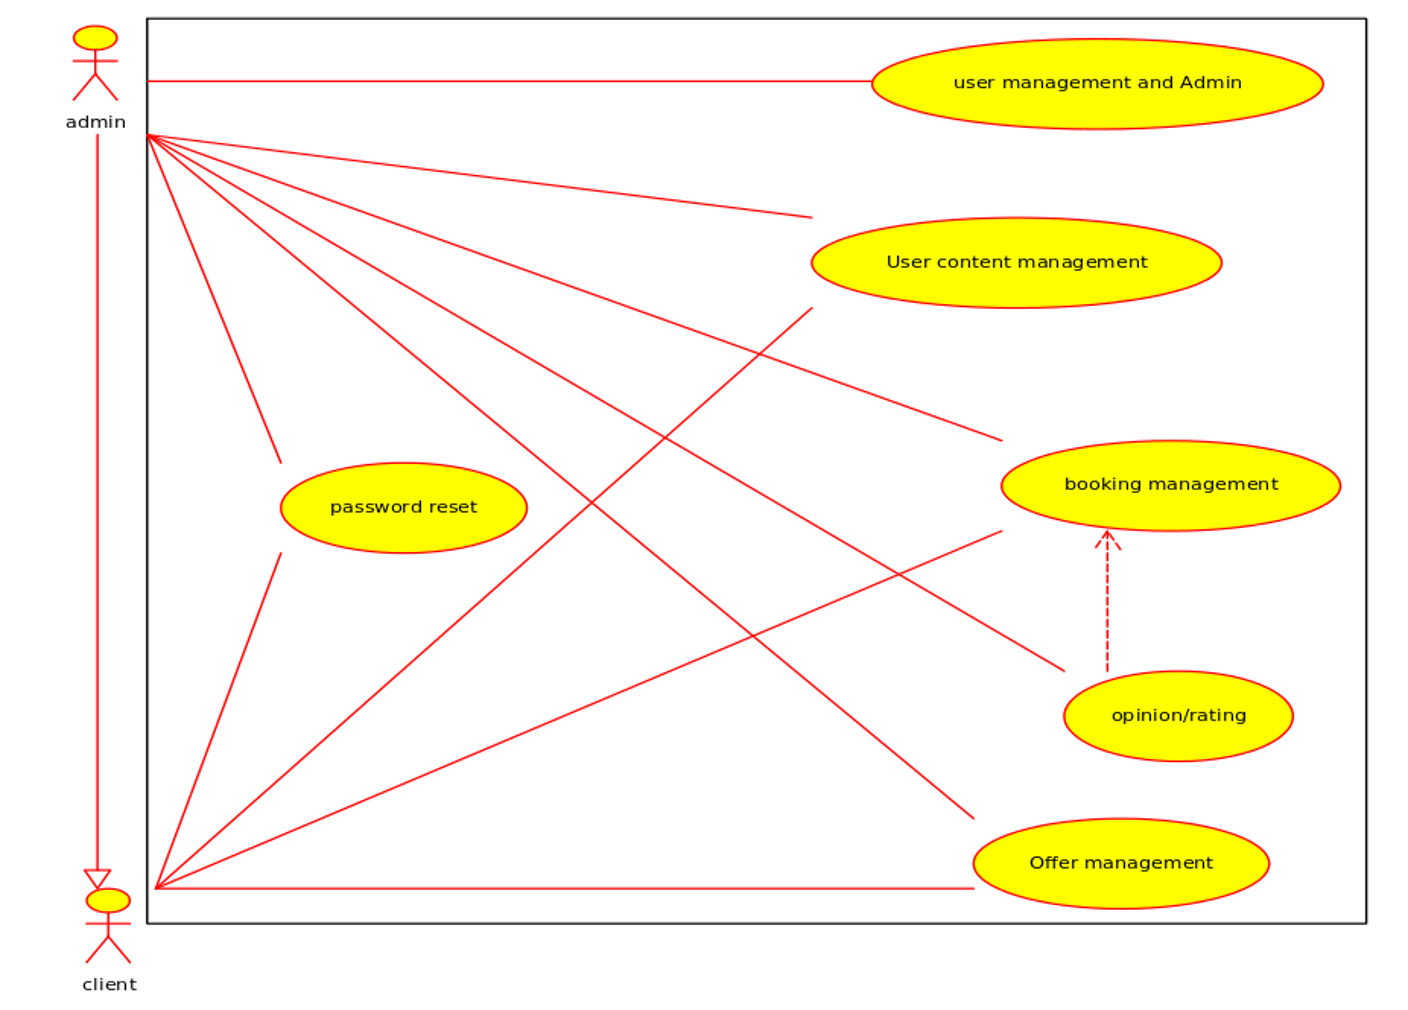
\includegraphics[scale=0.2]{../img/updated_use_case.jpg} 
		\caption{use case diagram in UML}
	\end{figure}
\end{frame}

\begin{frame}{Database Design}
%explain the problems about the database design 
%Mongo and it's advtanges and major disadvantages
\begin{figure}
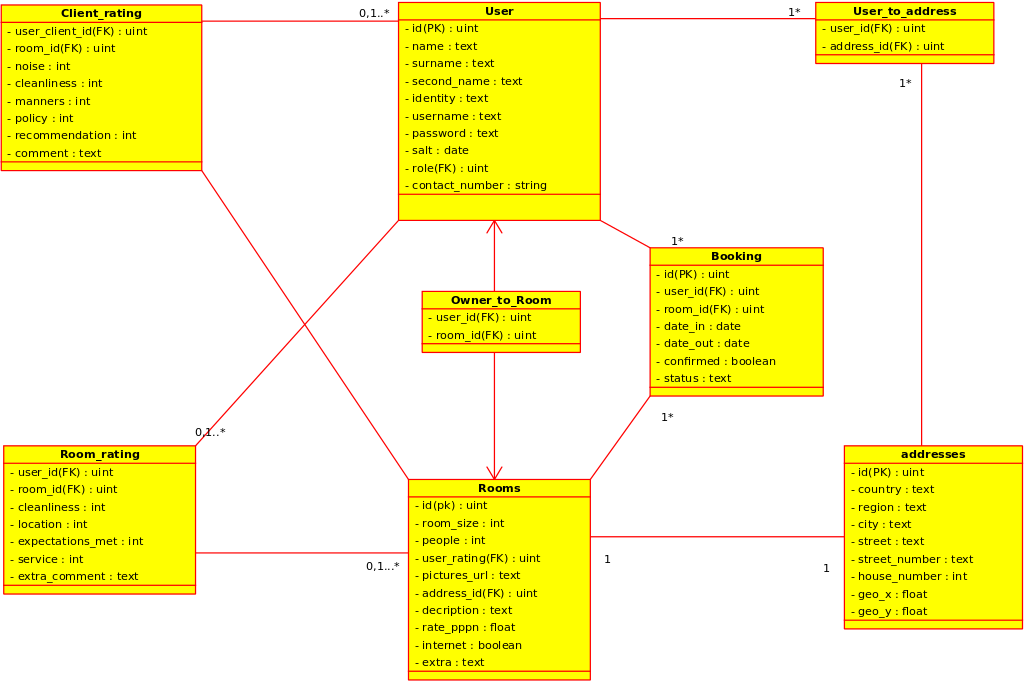
\includegraphics[scale=0.25]{../img/db.png} 
\end{figure}

\end{frame}

\begin{frame}{Architecture}
\begin{flushleft}
	\textbf{Three Tiered Architecture}
	\pause
	\begin{figure}
	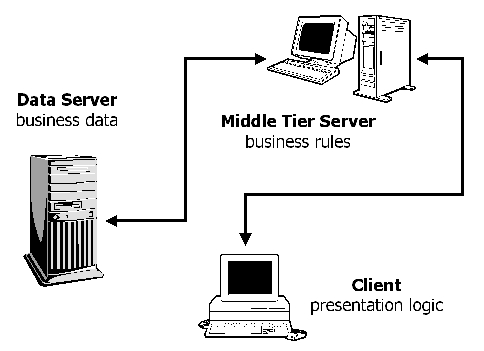
\includegraphics[scale=0.4]{3508f3.jpg} 
	\caption{simplified 3-tiered architecture}
	\end{figure}
	
\end{flushleft}
\end{frame}

\begin{frame}
\textbf{Design Patterns}
\pause
\begin{figure}
		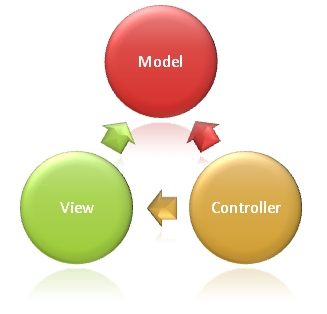
\includegraphics[scale=0.4]{27.jpg} 
		\end{figure}
	\begin{itemize}
		\item Model : Data to be presented/changed
		\item View : How the data is presented to the client
		\item Controller : interface between Model and View 
	\end{itemize}
	\textbf{Protocols and format}
	\begin{itemize}
		\pause
		\item \textbf{Re}presentational \textbf{S}tate \textbf{T}ransfer%explain that HTTP is used and why not soap
		\item HTTP(S) as the message exchange protocol  
		\item JSON as message format%explain HATEOAS principle
		%Hypertext As The Engine Of Application State
	\end{itemize}
\end{frame}
\begin{frame}{Technologies}
	\begin{flushleft}
	\textbf{MEAN}
	\begin{itemize}
		\pause
		\item Mongo DB 	: Database 
		\pause
		\item Express JS : development framework
		\pause
		\item Angular JS : presentation (single page apps)
		\pause
		\item Node JS  : back-end 
	\end{itemize}
	\pause
	\textbf{Additionally}
		\begin{itemize}
		\item OpenSSL%as a security feature
		\item CSS%for display 
		\end{itemize}
	\textbf{caveats}\\
	\pause
	Mongo DB might be substituted for a SQL database \\
	Angular JS might be substituted for EJS
	\end{flushleft}
\end{frame}

\begin{frame}{TODO/Problems}
	\textbf{TODO}\\
		\begin{itemize}
		\item API
		\item WWW server(might not happen)
		\end{itemize}
	\textbf{Problems}
	\begin{itemize}
		\item document store database (Mongo)
		\item relative anonymity
		\item security
		\item Graphical Interface
	\end{itemize}
\end{frame}

\end{document}